\section{半正定松弛与原解恢复}
\label{sec:opt-con-sdp-relaxation}

前面的算法大多依赖凸性：KKT条件的充分性、强对偶、内点法的中心路径，都在凸问题上才有完整的保证。许多实际问题却是非凸的二次问题，例如变量只能取$\pm1$的划分问题。本节研究一种把这类问题转成前面已经会解的半正定规划的办法：先把变量“提升”成矩阵，使二次式变成线性式，再删去唯一非凸的约束，得到一个凸的松弛问题；松弛解给出原最优值的界，但不一定是原问题的解，还需要恢复成原问题的可行候选并检验。这里改变的是候选的表示与可行集合，求解既定半正定规划的算法沿用第~\ref{sec:opt-con-interior-point}节。

\subsection{二次模型的提升与松弛}
\label{sec:opt-con-lifting}

\paragraph{精确提升}
考虑二次目标与二次约束的问题
\begin{equation}
\label{eq:opt-con-qcqp}
  \min_{\bm x\in\mathbb R^d}\ \bm x^\top\bm Q_0\bm x+2\bm q_0^\top\bm x+r_0\quad\text{s.t.}\quad\bm x^\top\bm Q_i\bm x+2\bm q_i^\top\bm x+r_i\leq0\ (i=1,\dots,m),
\end{equation}
其中$\bm Q_i$对称但不必半正定，问题一般非凸。关键观察是$\bm x^\top\bm Q\bm x=\langle\bm Q,\bm x\bm x^\top\rangle$：若引入矩阵变量$\bm X=\bm x\bm x^\top$，每个二次式都变成关于$(\bm x,\bm X)$的线性式$\langle\bm Q_i,\bm X\rangle+2\bm q_i^\top\bm x+r_i$。为了把$\bm x$与$\bm X$绑在一起，使用块矩阵
\[
  \bm Y=\begin{bmatrix}1&\bm x^\top\\\bm x&\bm X\end{bmatrix}\in\mathbb S^{d+1}.
\]
若$\bm X=\bm x\bm x^\top$，则$\bm Y=(1,\bm x^\top)^\top(1,\bm x^\top)$是半正定的秩一矩阵。反过来，若$\bm Y\succeq\bm0$、$\operatorname{rank}\bm Y=1$且左上角为$1$，则$\bm Y=\bm v\bm v^\top$，$v_1^2=1$；不妨$v_1=1$（否则把$\bm v$取负），于是$\bm x$等于$\bm v$的其余分量，$\bm X=\bm x\bm x^\top$。所以问题~\eqref{eq:opt-con-qcqp}精确地等价于关于$\bm Y$的线性目标、线性约束，加上$\bm Y\succeq\bm0$与$\operatorname{rank}\bm Y=1$。半正定与秩一两个条件共同保证新变量来自同一个原变量；非凸性全部集中到了秩一约束上。

\paragraph{删去秩一约束}
删去$\operatorname{rank}\bm Y=1$，保留$\bm Y\succeq\bm0$与左上角为$1$，就得到原问题的\term{半正定松弛}（semidefinite relaxation），它是一个半正定规划。由Schur补（引理~\ref{lem:opt-con-schur}），$\bm Y\succeq\bm0$等价于$\bm X-\bm x\bm x^\top\succeq\bm0$：松弛允许$\bm X$比真实乘积$\bm x\bm x^\top$“大”一个半正定矩阵。每个原可行点$\bm x$按$\bm X=\bm x\bm x^\top$映入松弛的可行域，且目标值不变，所以松弛的可行域包含原问题的全部候选，松弛最优值是原最优值的下界（对最大化问题则是上界）。

\begin{example}[最大割的半正定松弛]
\label{ex:opt-con-maxcut}
给定无向图的顶点$1,\dots,n$与边权$w_{a,b}\geq0$，把顶点分成两组，最大化跨组边的权重和，称为\term{最大割}（maximum cut）问题。用$x_a\in\{\pm1\}$表示顶点所在的组，边$(a,b)$跨组时$(1-x_ax_b)/2=1$，否则为$0$。约束$x_a\in\{\pm1\}$就是二次等式$x_a^2=1$。问题为
\[
  \max_{\bm x}\ \sum_{(a,b)\in E}w_{a,b}\frac{1-x_ax_b}{2}\quad\text{s.t.}\quad x_a^2=1.
\]
这里没有一次项，可直接用$\bm X=\bm x\bm x^\top$提升：目标变为$\sum w_{a,b}(1-X_{a,b})/2$，约束变为$X_{a,a}=1$。删去秩一约束，松弛为$\max\sum w_{a,b}(1-X_{a,b})/2$、$X_{a,a}=1$、$\bm X\succeq\bm0$。

取三角形图（三条边，权重均为$1$）。任何划分都至多切断两条边，最大割为$2$。松弛中，$\bm X\succeq\bm0$蕴含$\bm1^\top\bm X\bm1=3+2(X_{1,2}+X_{1,3}+X_{2,3})\geq0$，于是目标$\frac12(3-\sum X_{a,b})\leq\frac12(3+\frac32)=\frac94$；取全部非对角元为$-\frac12$，$\bm X=\frac32\bm I-\frac12\bm1\bm1^\top$的特征值为$0,\frac32,\frac32$，可行且达到$\frac94$。松弛值$9/4$严格大于真实最优值$2$，松弛解的秩为$2$，不对应任何$\pm1$向量。
\end{example}

\paragraph{与线性松弛的比较}
第~\ref{chap:opt-linear-programming}章的线性规划松弛把整数变量放宽到区间，同样扩大了候选集合、给出单侧的界。两者回答的是同一类问题，代价却不同：线性松弛保留$n$个变量，半正定松弛引入$O(n^2)$个矩阵元素和一个半正定约束，求解需要第~\ref{sec:opt-con-barrier-method}小节中代价较高的矩阵牛顿系统。对二次目标与$\pm1$变量，半正定松弛的界往往比简单的线性松弛紧，但更紧的界不意味着更低的计算成本；问题规模大时，存储和分解$\bm X$可能成为瓶颈。

也有松弛恰好精确的情形。例~\ref{ex:opt-con-sdp-eigen}中的$\min\langle\bm C,\bm X\rangle$、$\operatorname{tr}\bm X=1$、$\bm X\succeq\bm0$，正是非凸问题$\min\bm x^\top\bm C\bm x$、$\lVert\bm x\rVert_2^2=1$的半正定松弛；松弛最优解$\bm v\bm v^\top$秩为一，松弛值等于原最优值$\lambda_{\min}(\bm C)$。

\subsection{解的恢复与结果检验}
\label{sec:opt-con-rounding}

\paragraph{秩一时直接提取}
若松弛的最优解满足秩一条件，就可以按上一小节的论证提取$\bm x$：对$\bm Y$作特征分解，取最大特征值$\sigma_1$对应的单位特征向量$\bm v$，令$\bm x$为$\sqrt{\sigma_1}\bm v$缩放到首分量为$1$后的其余分量；然后逐条核对原约束~\eqref{eq:opt-con-qcqp}。数值求解给出的$\bm Y$只是近似秩一（第二大特征值很小但不为零），这时提取出的$\bm x$可能有微小违约，也必须按原约束检查。图~\ref{fig:opt-con-sdp-rounding}(a)是一个秩一的例子：四个顶点的圈（边$12,23,34,41$，权重为$1$）是二部图，最大割为$4$；松弛目标$\sum(1-X_{a,b})/2\leq4$（因为$X_{a,b}\geq-1$），而$\bm x=(1,-1,1,-1)^\top$的$\bm x\bm x^\top$达到$4$，所以松弛精确，解为秩一。

\paragraph{高秩时的随机舍入}
一般的松弛解秩大于一，需要针对任务设计恢复规则。最大割有一个经典的\term{随机超平面舍入}（random hyperplane rounding）方法。把松弛解分解为$\bm X=\bm V^\top\bm V$，$\bm V$的第$a$列$\bm v_a$是单位向量（因为$X_{a,a}=1$），$X_{a,b}=\langle\bm v_a,\bm v_b\rangle$。随机取一个方向$\bm r$（如标准正态向量），令$x_a=\operatorname{sign}\langle\bm r,\bm v_a\rangle$，即用过原点、以$\bm r$为法向的超平面把这些向量分成两组。两个单位向量被分开的概率等于它们的夹角除以$\pi$，所以舍入得到的割值期望为
\[
  \mathbb E\Bigl[\sum_{(a,b)\in E}w_{a,b}\frac{1-x_ax_b}{2}\Bigr]=\sum_{(a,b)\in E}w_{a,b}\frac{\arccos X_{a,b}}{\pi}.
\]
在非负权重下，Goemans与Williamson证明这个期望不低于松弛值的$0.878$倍，因而也不低于最大割的$0.878$倍\scite{goemans1995maxcut}。这是针对最大割的结论，依赖目标的特殊形式；不能预设任意二次问题都有保证精度的恢复办法。

回到三角形：$X_{a,b}=-\frac12$对应三个在平面内两两成$120^\circ$的单位向量（图~\ref{fig:opt-con-sdp-rounding}(b)）。每条边被分开的概率为$(2\pi/3)/\pi=\frac23$，期望割值为$3\times\frac23=2$。实际上，任何不经过这三个向量的超平面都恰好把其中一个与另外两个分开，每次舍入都得到割值$2$，正是最大割。

\begin{figure*}[!htbp]
  \centering
  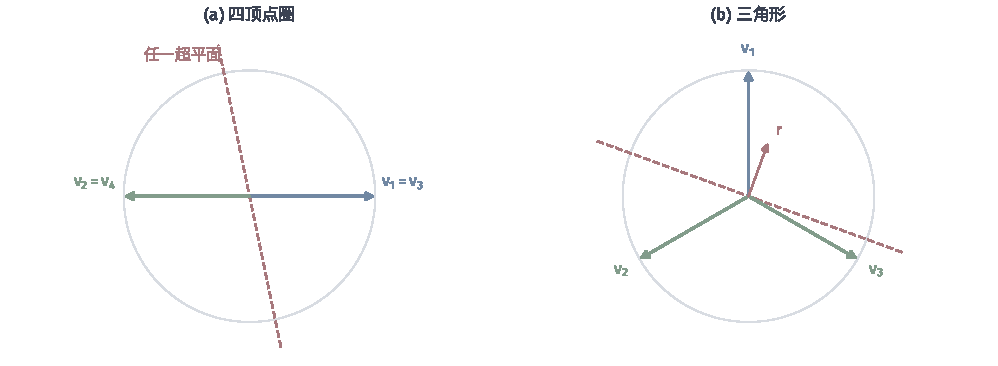
\includegraphics[width=169mm]{figures/03-optimization-evolution-and-signals/01-optimization/matplotlib/c5-sdp-rounding/figure.pdf}
  \caption{最大割半正定松弛的向量表示$X_{a,b}=\langle\bm v_a,\bm v_b\rangle$。(a) 四顶点圈：松弛解是秩一的，$\bm v_1=\bm v_3$与$\bm v_2=\bm v_4$方向相反，任何超平面（红色虚线）都给出割值$4$，与松弛值相等。(b) 三角形：三个单位向量两两成$120^\circ$，松弛值为$9/4$；以随机方向$\bm r$为法向的超平面把$\bm v_1$（蓝）与$\bm v_2,\bm v_3$（绿）分开，得到割值$2$，即最大割。}
  \label{fig:opt-con-sdp-rounding}
\end{figure*}

\paragraph{用上下界报告结果}
恢复步骤只产生候选。对实际得到的原始可行候选，其目标值给出最大割的一个下界（最大化问题）；松弛给出上界。二者合起来报告一个区间：三角形的最大割位于$[2,9/4]$，舍入候选的值$2$恰为下端点，区间宽度反映的是松弛本身的间隙，而不是舍入的损失。

这里的上界要可信。数值求解松弛问题只得到近似解，近似解的目标值可能略高或略低于真正的松弛最优值，直接拿来当上界并不严格。可靠的做法是给出一个对偶可行点。对最大割，目标可写成$\frac14\langle\bm L,\bm X\rangle$，其中$\bm L$是图的Laplace矩阵（对角元为加权度数，非对角元为$-w_{a,b}$）；对任何$\bm X\succeq\bm0$、$X_{a,a}=1$，$\frac14\langle\bm L,\bm X\rangle\leq\frac14\lambda_{\max}(\bm L)\operatorname{tr}\bm X=\frac n4\lambda_{\max}(\bm L)$。三角形的$\bm L=3\bm I-\bm1\bm1^\top$，$\lambda_{\max}=3$，上界$\frac34\cdot3=\frac94$，与松弛值一致。这类由对偶可行点构造的界，不受松弛求解误差的影响。

最后，三种误差应分别记录：求解松弛问题的数值误差（由松弛问题自身的原始—对偶残差控制）；松弛间隙，即放宽可行域造成的松弛值与原最优值之差（三角形中为$1/4$，四顶点圈中为零）；以及恢复的损失或失败，包括恢复候选违反原约束、需要修复，或目标值低于原最优值。三者来源不同，不能互相抵消或替代。最终的输出必须回到原始的非凸问题：一个经过原约束检验的候选，以及一个注明来源的界。
